% FairMind-E position paper for GREENS 2027 (ICSE 2027 workshop).
% Single-anonymous: authors shown. IEEE conference format, 5 pages max.
% Adapted from ../ccai2026/preprint.tex; figures come from analysis/make_figures.py.

\documentclass[10pt,conference]{IEEEtran}

\usepackage[utf8]{inputenc}
\usepackage[T1]{fontenc}
\usepackage{cite}
\usepackage{amsmath}
\usepackage{graphicx}
\usepackage{booktabs}
\usepackage{url}
\usepackage[hidelinks]{hyperref}
\graphicspath{{../ccai2026/figures/}}

\newcommand{\sysname}{FairMind-E}

\begin{document}

\title{Release Gates Should Ask\\Where the Carbon Number Came From}

\author{\IEEEauthorblockN{Adhithya Rajasekaran}
\IEEEauthorblockA{Axonome\\
adhi.r@axonome.xyz\\
ORCID 0009-0004-1682-7958}}

\maketitle

\begin{abstract}
Green software practice increasingly puts a carbon number in front of a release
decision: a carbon budget, a readiness level, or a risk rating. None of these
gates asks whether the number itself can be trusted. We argue that the
\emph{provenance} of an environmental claim should be a first-class release
criterion, and we report on \sysname, an environmental release gate shipped
inside FairMind, an open-source AI governance platform. A provenance-derived
confidence score crossed with an impact tier resolves to \emph{go},
\emph{conditional\_go}, or \emph{no\_go}, and blocks the platform's
deployment-approval workflow. In a measurement study over four workloads, five
iterations each, a software power tracker and an analytic FLOP model assessed
every run and disagreed on magnitude by 123--169 percent MAPE, depending on
which is taken as reference. One routine mitigation failed outright: casting a
fine-tune to \texttt{bfloat16} on a host with no optimised kernel made it 46
times slower, and the tracker estimated roughly 41 times the energy. A gate
that accepts declared mitigations would have logged a reduction that never
happened.
\end{abstract}

\begin{IEEEkeywords}
green software, sustainable AI, release engineering, carbon measurement,
evidence quality, AI governance
\end{IEEEkeywords}

\section{Position}

Software teams are being asked to account for the energy and carbon of the AI
systems they ship. Standards bodies are building the measurement layer:
quantification-methods inventories~\cite{cen18145}, sustainability
overviews~\cite{iso20226}, and a G7-commissioned inventory of thirteen
measurement and reporting initiatives~\cite{g7}. The EU AI Act anticipates
harmonised standards for reporting AI resource performance (Article~40) and
requires general-purpose model documentation to state known or estimated energy
consumption (Annex~XI)~\cite{aiact}. None of these instruments says how the
\emph{quality} of an environmental claim should condition a deployment
decision.

Proposed carbon-aware gates decide on magnitude. Carbon-aware governance gates
embed carbon budgets and record provenance only in audit logs~\cite{cagg};
sustainability pyramids gate on readiness levels~\cite{gtrace}; risk
integrations treat AI carbon as one risk dimension~\cite{tkachenko}. Yet
measurement research shows reliability varies sharply with disclosure:
metadata-completeness tiers across 5{,}227 public models span roughly
$1.2\times$ to $2\times$ estimation error~\cite{huggingcarbon}, and spend-based
fallbacks in tiered Scope~3 accounting overestimate by
10--40$\times$~\cite{scope3}. Recent work acts on the \emph{statistical spread}
of an estimate, through conformal calibration inside a carbon budget
gate~\cite{greensarc} or confidence-gated filtering of emissions
predictions~\cite{trustpems}. None acts on \emph{where the number came from}, so
a precise-looking figure from a weak source passes every published gate while
sitting comfortably under budget.

Our position is narrow: \textbf{for green software engineering, evidence
quality, not only impact magnitude, should gate a release.} The idea is old in
life-cycle assessment, where pedigree matrices grade the provenance of an
inventory figure~\cite{weidema} and the NUSAP pedigree qualifies
uncertainty~\cite{nusap}; recent work recommends indicator-style disclosure for
AI-assisted footprinting but proposes no score, threshold, or
gate~\cite{credible}. We bring it into the release pipeline, where software
engineers already make go or no-go decisions.

\section{Mechanism}

\paragraph{Provenance classes and confidence} Every assessment declares its
measurement source, normalised to one of five provenance classes with bounded
confidence: \emph{measured} (hardware telemetry; 0.85--1.00),
\emph{tool\_estimated} (software power trackers; 0.60--0.85),
\emph{vendor\_reported} (cloud-provider figures; 0.40--0.60), \emph{manual}
(analytic FLOP estimates; 0.20--0.40), and \emph{unknown} (0.0). A
caller-supplied score is honoured but capped by its provenance class, and
unknown provenance forces 0.0 whatever score is claimed. Provenance is reported
separately from quantified uncertainty, so a narrow interval cannot launder a
weak source.

\paragraph{Tiers and the decision matrix} Metrics map to low, medium, or high
impact per lifecycle phase, using location-based carbon so market instruments
cannot lower a gate outcome. Confidence bands (\emph{high} $\geq 0.70$;
\emph{moderate} $0.35 \leq c < 0.70$; \emph{low} $0 < c < 0.35$;
\emph{undisclosed} $c = 0$) cross with impact tiers into the matrix in
Fig.~\ref{fig:main}(b). Confidence 0.0 short-circuits to \emph{no\_go}: an
undisclosed claim never passes. A \emph{conditional\_go} cannot be approved
until it carries a dated, owned mitigation or an explicit exception with owner,
expiry, and rationale, so reviewer overrides are auditable rather than
informal. Six controls (ENV-1 to ENV-6: boundary, energy accounting, dual
location and market carbon, per-functional-unit efficiency, evidence confidence
with disclosed uncertainty, and mitigation or exception) define coverage.
Disclosed offsets are recorded but never subtracted and never improve a gate
outcome.

\section{Implementation in a release pipeline}

\sysname{} ships inside FairMind rather than as a standalone proposal. The
decision engine is a framework-agnostic Python package with 57 unit tests
covering every matrix cell, band boundary, provenance cap, and the
undisclosed-evidence short-circuit. Assessments persist as versioned governance
evidence. A release gate hooks the platform's deployment-approval workflow and
returns HTTP 409 with the blocking reason when the latest assessment is
\emph{no\_go} or an unmitigated \emph{conditional\_go}, the same way a failing
test blocks a merge. Reviewers see the matrix position, control coverage,
mitigations, and version trail; disclosures export in a shape aligned with the
European climate reporting standard~\cite{csrd}.

A 14-case hand-labelled fixture set spanning all matrix cells, mitigation
states, exception paths, and offset disclosures serves as a conformance test:
the implementation reproduces 14/14 labels. Because the same author wrote the
fixtures, labels, and engine, this shows only that the code implements the
stated policy, not that the policy decides correctly.

\section{Measurement study}

\begin{figure}[t]
  \centering
  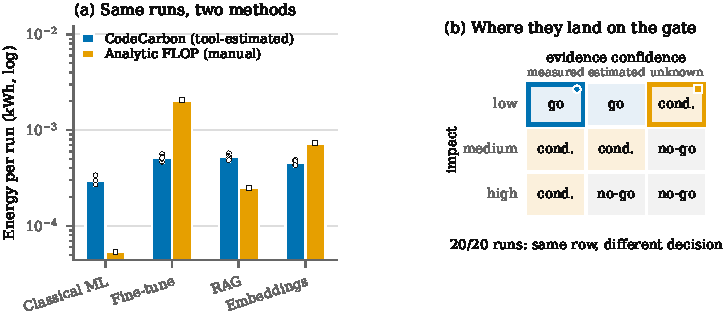
\includegraphics[width=\linewidth]{fig1_provenance_decides.pdf}
  \caption{Four workloads, five iterations each, every run assessed twice.
  (a) The methods disagree by 123--169 percent MAPE depending on reference;
  points are iterations, bars their means. (b) Where those runs land. Both put
  every run in the same \emph{low} row, so the column moved because provenance
  moved. The panel illustrates the mechanism; it does not validate it.}
  \label{fig:main}
\end{figure}

Four workloads (classical ML training, transformer fine-tune, RAG inference,
batch embeddings) ran five iterations each on one host (Apple M1 Pro; seed
1337; warm-up discarded). Every run was assessed by a software power tracker
(\emph{tool\_estimated}) and a documented analytic FLOP model
(\emph{manual}); cloud billing was also requested but lags execution, so its 20
records are explicit ``unavailable'' entries rather than invented figures. All
runs were replayed through the production engine, not a reimplementation.

\paragraph{The empirical finding is the disagreement} MAPE is 122.6 percent
with the tracker as reference and 169.1 percent with the FLOP model as
reference, ranging from 52 to 298 percent by workload, with Bland-Altman limits
of agreement from $-1.15{\times}10^{-3}$ to $1.79{\times}10^{-3}$~kWh
(Fig.~\ref{fig:main}(a)). Two methods a practitioner might reasonably choose
disagree by more than a factor of two on the same run.

\paragraph{The decision split is a policy consequence} The tracker maps to
confidence 0.72 (\emph{high} band, \emph{go}); the FLOP model to 0.30
(\emph{low} band, \emph{conditional\_go}), on all 20 runs. Since confidence is
constant per provenance class and the tier stayed \emph{low}, the split follows
from the policy and is not independent evidence for it. What it does show is
that the mechanism runs end to end on real runs, and that a magnitude-only gate
is structurally blind to the split.

\begin{figure}[t]
  \centering
  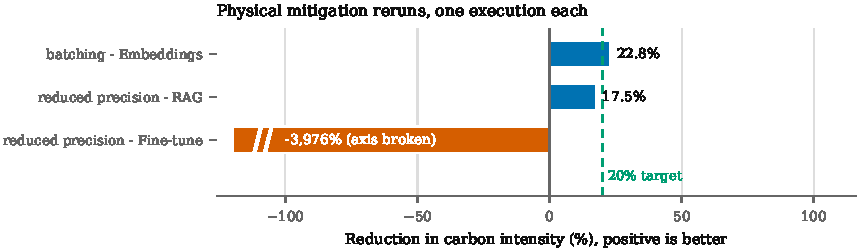
\includegraphics[width=\linewidth]{fig2_mitigations.pdf}
  \caption{Mitigation outcomes by what was executed. Hatched bars are
  accounting scenarios recomputed against a \emph{placeholder} emission-factor
  table with no rerun: illustrative arithmetic, not measurements. Solid bars
  are the three physical reruns. The \texttt{bfloat16} fine-tune went from
  62.7\,s to 2887.6\,s; its bar is truncated.}
  \label{fig:mitigations}
\end{figure}

\paragraph{Mitigations} Only three mitigations were physical reruns
(Fig.~\ref{fig:mitigations}); region and time shifts recompute one measured run
against placeholder factors and are reported as arithmetic, not reductions.
Batching cut intensity 22.8 percent and a reduced-precision cast on RAG 17.5
percent. The third inverted: casting the fine-tune to \texttt{bfloat16} made it
46 times slower on a host with no optimised kernel, and the tracker estimated
roughly 41 times the energy. The runtime regression is measured directly; the
energy figure inherits the tracker's power model. ``We reduced precision,
therefore we cut carbon'' is a routine and plausible claim; here it was false
in the harmful direction. This is why ENV-6 requires a mitigation to be
re-measured rather than declared.

\section{Implications for green software engineering}

\paragraph{Make measurement the cheapest path to release} When evidence
quality gates a release, a team that cannot substantiate its number cannot ship
unconditionally, so measuring becomes cheaper than arguing. This does not cut
emissions by itself; it makes reported reductions verifiable, and therefore
something a team can act on.

\paragraph{Treat mitigations like code changes} A mitigation is a claim about a
change. Like a performance fix, it should be re-measured in the pipeline before
it is credited, because the effect of a precision cast or a batching change
depends on the hardware and kernels underneath.

\paragraph{Open questions for the workshop} Is the provenance hierarchy the
right one, and how should it be calibrated against an independent power
reference? Which confidence bands should a CI pipeline use when only software
estimates exist, as on most developer hardware? And how should overrides be
audited so that \emph{conditional\_go} does not become the new default?

\paragraph{Limitations} The host exposes no hardware energy counters, so the
tracker fell back to load-based estimation: the study compares an estimate with
an estimate and never claims the \emph{measured} class. Benchmark workloads
exercise only the low-impact row, the FLOP model uses placeholder constants,
and confidence is not yet calibrated against an independent power reference;
that calibration, and a 15-reviewer expert panel already designed, are the next
steps. Code, run data, and analysis scripts are public in the FairMind
repository (\url{https://github.com/adhit-r/fairmind}, release v0.3.0-alpha,
doi:10.5281/zenodo.24043235).

\section*{Acknowledgment}
FairMind is developed at Axonome, where the author works; the work received no
external funding. Generative AI tools (Claude, through Claude Code) assisted
with code and drafting; the author reviewed all output and is responsible for
the content.

\begin{thebibliography}{99}
\footnotesize
\bibitem{cen18145} CEN/CLC/TR 18145:2025, \emph{Environmentally sustainable
artificial intelligence: quantification methods inventory}, 2025.
\bibitem{iso20226} ISO/IEC TR 20226:2025, \emph{Artificial intelligence:
environmental sustainability aspects}, 2025.
\bibitem{g7} G7 French Presidency, \emph{Overview of initiatives for the
measurement and monitoring of energy and resource use of AI models}, May 2026.
\bibitem{aiact} Regulation (EU) 2024/1689 (Artificial Intelligence Act),
Article 40 and Annex XI \S1(2d), 2024.
\bibitem{cagg} ``Carbon-aware governance gates: embedding carbon budgets, energy
provenance, and sustainability-aware validation in governance layers,''
arXiv:2602.19718v2, 2026.
\bibitem{gtrace} ``G-TRACE: an AI sustainability pyramid for carbon-aware
governance readiness,'' arXiv:2511.04776v3, 2026.
\bibitem{tkachenko} N. Tkachenko, ``Sustainable integration of frontier AI in
banking,'' \emph{Journal of Financial Compliance}, 2025.
\bibitem{huggingcarbon} ``Hugging Carbon: estimation reliability tiers for the
carbon footprint of 5,227 public models,'' arXiv:2605.01549v2, 2026.
\bibitem{scope3} ``A four-tier Scope 3 methodology for AI inference under
CSRD,'' arXiv:2606.10660, 2026.
\bibitem{greensarc} ``Green SARC: predictive cost and carbon governance for
agentic AI with split-conformal calibration,'' arXiv:2606.15954, 2026.
\bibitem{trustpems} ``Trust-aware predictive emissions monitoring:
confidence-gated filtering of industrial emissions estimates,''
arXiv:2606.06156, 2026.
\bibitem{weidema} B. P. Weidema and M. S. Wesn\ae s, ``Data quality management
for life cycle inventories: an example of using data quality indicators,''
\emph{Journal of Cleaner Production}, vol. 4, no. 3--4, pp. 167--174, 1996.
\bibitem{nusap} S. O. Funtowicz and J. R. Ravetz, \emph{Uncertainty and Quality
in Science for Policy}. Dordrecht: Kluwer, 1990.
\bibitem{credible} ``Criteria for credible AI-assisted carbon footprinting
systems,'' arXiv:2509.00240, 2025.
\bibitem{csrd} Directive (EU) 2022/2464 (Corporate Sustainability Reporting
Directive) and ESRS E1, Climate change, 2023.
\end{thebibliography}

\end{document}
